\part{Ряды Фурье}
\section{Основные определения}

\begin{Def}
	Пусть функция $f(x)$ определена на $\bb{R}$ и $\exists T > 0, \;\\
	\forall x \in \bb{R} f(x+T) = f(x)$. Тогда функция $f(x)$ называется $T-$периодической функцией, а $T$ \textendash её период. Причём:\\
	$\forall k \in \bb{Z} \backslash \{0\} \quad T' = kT$ тоже период $f(x),$ т.к. $\forall x \in \bb{R} f(x+T') = f(x)$
\end{Def}

Пример:\\
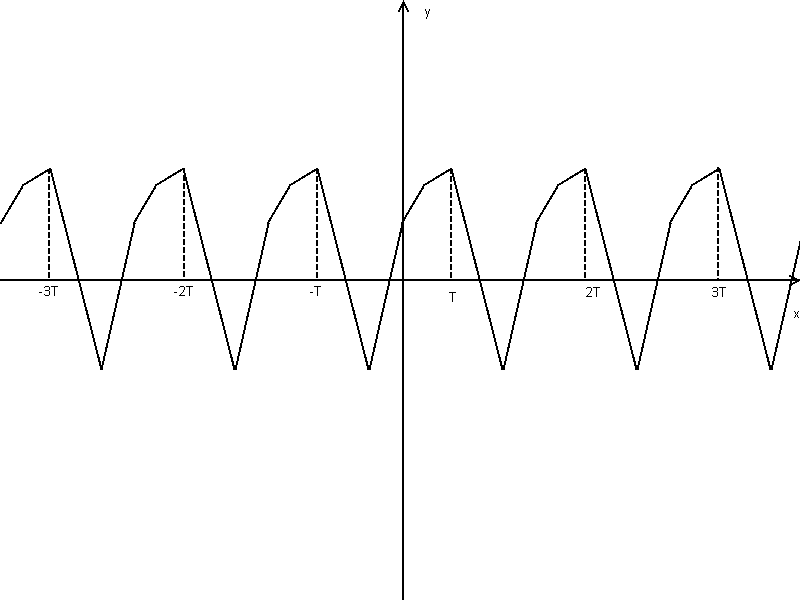
\includegraphics[width=1.0\textwidth]{pictures/5_1.png}

\begin{Note}
	Функция $f(x) = const$ периодична, причём период - любое число
\end{Note}

\begin{Def}
	Пусть функция $f(x)$ определена на $\bb{R}$, $T$-периодична, $T > 0$ и $\forall [a;b] \; \exists \int\limits_{a}^{b}f(x)dx$, тогда $f(x) \in R_T$ (функция $f(x)$ тоносится к классу периодично интегрируемых (или интегрируемых на периоде))%Здесь не помню, что должно стоять
\end{Def}

\begin{Lem}
	Пусть функция $f(x) \in R_T, \; T > 0$, тогда $\forall a \in \bb{R} \int\limits_{a}^{a+T}f(x)dx = \int\limits_{0}^{T}f(x)dx$
\end{Lem}

\begin{Proof}
	$\int\limits_{T}^{a+T}f(x)dx = [x = u + T \Rightarrow u \big|_{0}^{a}, du = dx] = [f(x) = f(u + T) = f(u)] = \int\limits_{0}^{a}f(u)du = -\int\limits_{a}^{0}f(x)dx$\\
	По аддитивности интегралов $\int\limits_{a}^{a+T} = \int\limits_{a}^{0} + \int\limits_{0}^{T} + \int\limits_{T}^{a+T} = \int\limits_{0}^{T}$
\end{Proof}

\begin{Def}(Тригонометрическая система функций)\\
	$u = \{1, \cos x, \sin x, \cos 2x, \sin 2x, \dots, \cos nx, \sin nx, \dots\}$ - тригонометрическая система функций
\end{Def}

\begin{Def}
	$T_n(x) = \sum\limits_{k=1}^{n} (a_k\cos kx + b_k\sin kx) + A$ - тригонометрический ряд
\end{Def}